\documentclass{kththesis}
\usepackage{csquotes} % Recommended by biblatex
\usepackage[style=numeric,sorting=none,backend=biber]{biblatex}
\usepackage[swedish]{babel}
\usepackage{graphicx}

\addbibresource{references.bib} % The file containing our references, in BibTeX format

\title{Find objects in real estate images with convolutional neural networks}
\alttitle{Hitta object i fastighetsbilder med convolutional neural networks}
\author{Oskar Råhlén och Sacharias Sjöqvist}
\email{orahlen@kth.se och sacsjo@kth.se}
\supervisor{Handledare}
\examiner{Examinator}
\programme{Degree project in Computer Science}
\school{School of Electrical Engineering and Computer Science}
\date{\today}

% Uncomment the next line to include cover generated at https://intra.kth.se/kth-cover?l=en
% \kthcover{kth-cover.pdf}

\begin{document}
% Frontmatter includes the title-page, abstracts and table-of-contents
\frontmatter

\titlepage

\begin{abstract}
  English abstract goes here.
\end{abstract}

\begin{otherlanguage}{swedish}
  \begin{abstract}
    Svenskt sammanfattning
  \end{abstract}
\end{otherlanguage}

\tableofcontents

% Mainmatter is where the actual contents of the thesis goes
\mainmatter

% Citera med \texttt{} och \parencite{}

\chapter{Introduktion}

Koppla första mening till titel.

söka på speicfika saker i en annons.
mysig inledning.

Deeplearning bildanalys - google grejer.

Ai och hur automatisering vuxit fram. 
Lite fakta på hur viktig sökfunktioner är för att hitta bostäder? Hur många sökningar /tidsenehet

Om folk enklare hittar bostad på ett mer effektivt sätt så effektiviseras hela köp och sälj processen och därmed hela marknaden.


  \section{Problemformulering}
  För att hitta nyckelord kopplade till en bild idag så behöver någon manuellt bestämma nyckelord till bilden. Uppgiften är tidskrävande och det är svårt att i efterhand producera relevanta nyckelord utan att gå igenom allt manuellt igen. 

  Det är också för bostadssökare tidskrävande att leta efter bostäder. Om man kan förfina sökningen än mer skulle detta effektivisera processen.

  Syftet med den här studien är att titta på hur maskininlärningsmetoder kan användas för att hitta relevanta nyckelord till bilder på lägenhetsannonser. 

  \section{Frågeställning}
  Går det med nuvarande verktyg inom maskininlärning hitta attribut i bilder från lägenhetsannonser?


  \section{Avgränsningar}
  Vilka avgränsningar vi gjort i datamängder, testpersoner samt modeller.

\chapter{Bakgrund}
  \section{Maskininlärning}
  En maskininlärningsalgoritm är en algoritm som kan lära sig och bli bättre från data \parencite{Goodfellow-et-al-2016}. Det kan beskrivas som ett datorprogram som kan följa en grupp med uppgifter T och lära sig med hjälp av erfarenhet E och dess prestanda P är mätbar. Maskininlärning hjälper oss att läsa problem som är för svåra för program skrivna och designade av människor att lösa. 

  Enligt \cite{Goodfellow-et-al-2016} är ett vanligt problem att lösa med maskininlärning klassificeringsproblem. Det innebär att bestämma vilken av k klasser en viss indata tillhör. För att lösa detta skapar man vanligtvis en funktion som tar in indata x och returnerar y, vilket är ett tal som representerar klassen. Det går även att returnera en sannolikhetsdistribution över alla klasser. Enligt \cite{Goodfellow-et-al-2016} så löses modern objektigenkänning med djupinlärning.

  En typ av algoritmer inom maskininlärning är supervised learning algorithms \parencite{Goodfellow-et-al-2016}. En sådan algoritm lär sig av data (erfarenhet E) som redan är uppmärkt med rätt klass. Detta kallas för labeled data. Det man vanligtvis gör är att man delar upp den märkta datan i ett träningsset och testset. Därefter tränar man algoritmen på sitt träningsset och testar sedan hur bra den fungerar, i form av fel (error) eller noggrannhet (accuracy), på sitt testset.

  Enligt \parencite{Goodfellow-et-al-2016} så är så kallade AI-kompletta problem,som objektigenkänning, bra att ha en baseline modell som är baserad på djupinlärning. Det är även bra att börja med ett CNN om indata består av bilder. 

  Man borde använda någon form av regularization. Där är dropout bra och fungerar i många tillfällen. Early stopping borde nästan alltid användas. Batch normalization kan användas istället för dropout, för att minska generaliseringsfel. 

  Om problemet är studerat förut så kan det vara bra att utgå ifrån modeller och algoritmer som redan har visats sig fungera bra. I bildigenkänning så är det till och med vanligt att man utgår ifrån samma vikter, så kallad transfer learning. Vanligtvis tränas då CNN upp på bilder från ImageNet. 

    \subsection{Neural networks}
    Neurala nätverk är en modell inom maskininlärning. Dess mål är att approximera en funktion f \parencite{Goodfellow-et-al-2016}. De är en viktig del av maskininlärningen och en specifik typ av feedforward network är convolutional neural networks, som är vanligt förekommande inom bildkategorisering. 

    Den nuvarande tekniken för objektigenkänning använder sig huvudsakligen av maskininlärning \parencite{krizhevsky_imagenet_2012}. För att öka dess prestanda så kan man samla in mer data, lära sig mer kraftfulla modeller eller använda sig av bättre tekniker för att undvika overfitting.

  \section{Convolutional Neural Network}
  Convolutional Neural Network är en typ av nätverk för indata som kan ses som ett rutnät \parencite{Goodfellow-et-al-2016}. I fallet om bilder så är det ett tvådimensionellt rutnät av pixlar. Det som gör CNN speciellt är att de använder sig av den linjära operationen convolution istället för vanlig matrismultiplikation i minst ett av sina lager.

  För en så avancerad uppgift som objektigenkänning så räcker det inte med stora mängder data, det behövs en modell med tidigare erfarenhet (prior knowledge) som tar korrekta antaganden om bilder. Detta gör convolutional neural networks (CNNs) bra \parencite{krizhevsky_imagenet_2012}. Jämfört med ett vanligt feedforward neural network med samma storlek på varje lager, så har CNNs färre anslutningar och färre parametrar, vilket gör att de blir enklare att träna.


  

    \subsection{Arkitekturer}
    Ett bra sätt att välja arkitektur är att att testa flera olika arkitekturer och frysa alla lager förutom det sista, och se resultatet \parencite{Goodfellow-et-al-2016}. Efter man hittat den bästa så tränar man alla lager.

  \section{Transfer Learning}
  Transfer Learning handlar om att överföra information mellan två olika området \parencite{oquab_learning_2014}. I datorseende (computer vision) handlar transfer learning huvudsakligen om att minska träningsprocessen genom att använda ett neuralt nätverk som redan är tränat på andra kategorier av bilder. Så man överför vikterna från ett tränat nätverk till ett nytt nätverk och anpassar det sedan för att kategorisera det man anser att kategorisera.

  \section{Fine-tuning och minska overfitting}
  Enligt \cite{krizhevsky_imagenet_2012} finns det minst två bra tekniker för att minska overfitting, data augmentation och dropout.

    \subsection{Data Augmentation}

    \subsection{Dropout}

\chapter{Metod}
Hur vi gått tillväga. Vilka dataset, hur implementation gått till (verktyg, klassificerare, parametrar), hur vi valt features.
Hur evalueringen har gått till (traning, test, validation set).

Vi vill mäta både precision och recall. Plotta en PR curve.

Vi kan även plotta hur precisionen har gått om i förhållande till mer data, för att skapa en uppfattning av om modellen kan bli bättre med mer data. Vanligtvis gör man detta i log-skala \parencite{Goodfellow-et-al-2016}. 

Gör även att göra en grid search på hyperparametrar.

Hur vi kan använda oss av preprocessing kan vi  läsa i kapitel 12 av Goodfellow.

\chapter{Resultat}
Presentation av resultatet från våra olika tekniker och evalueringar. i tabeller och grafer. Även beräkningstid. 

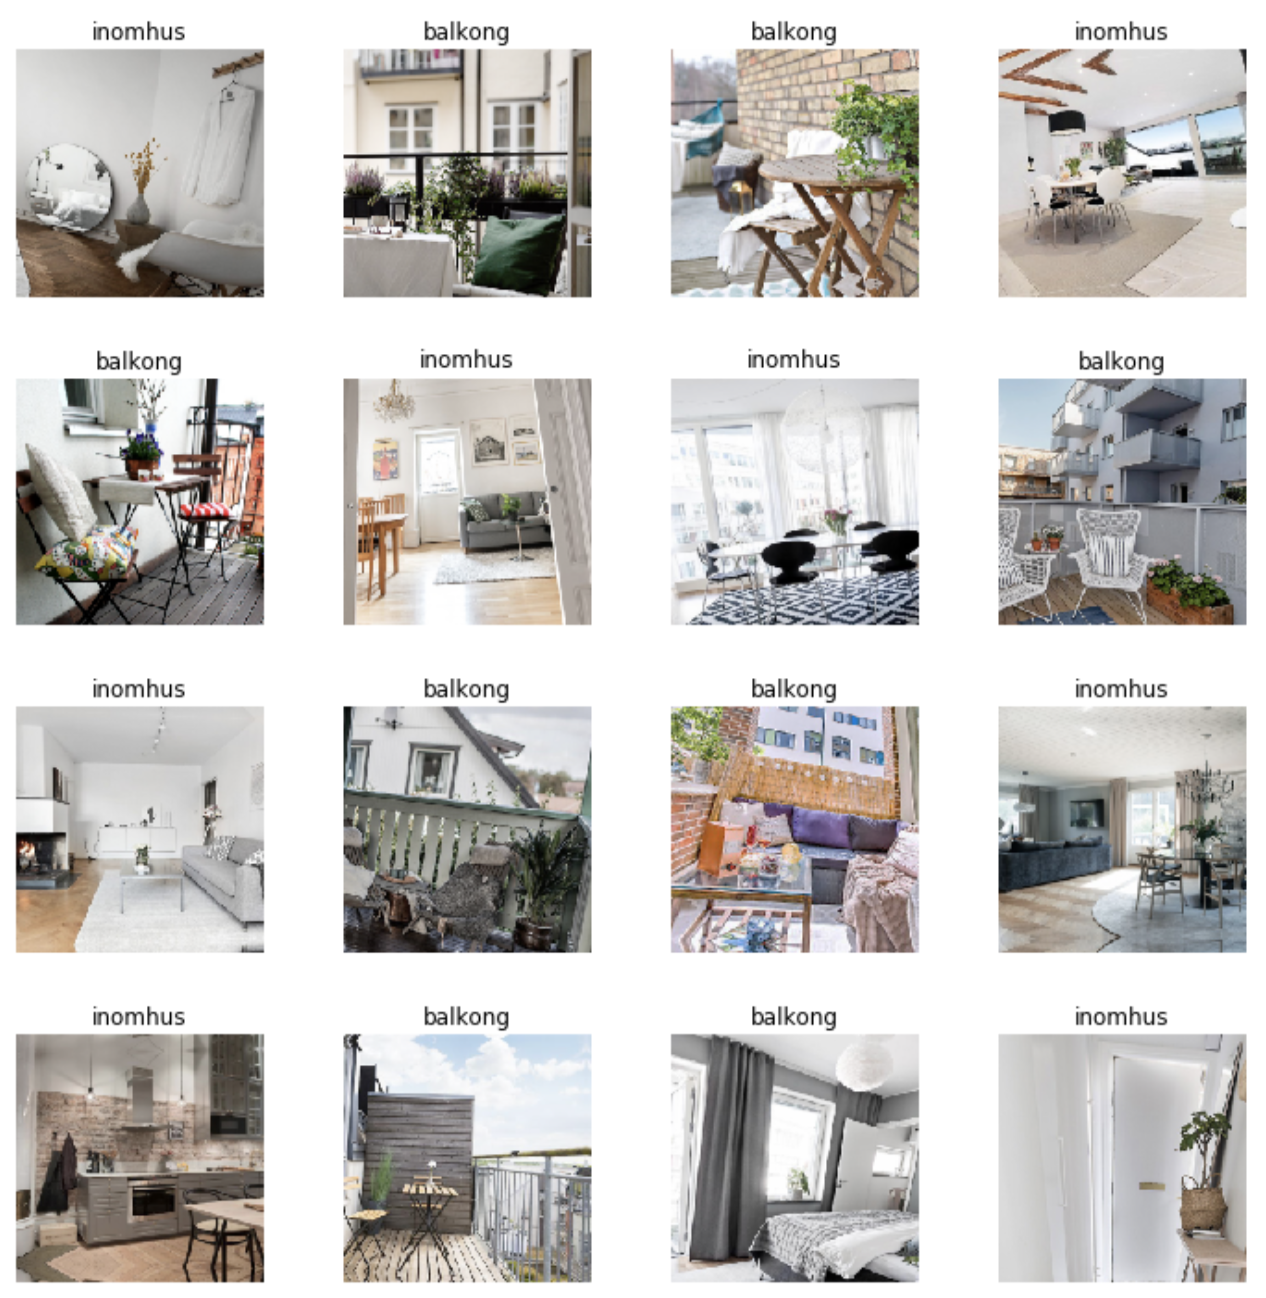
\includegraphics[width=10cm]{../images/1.png}

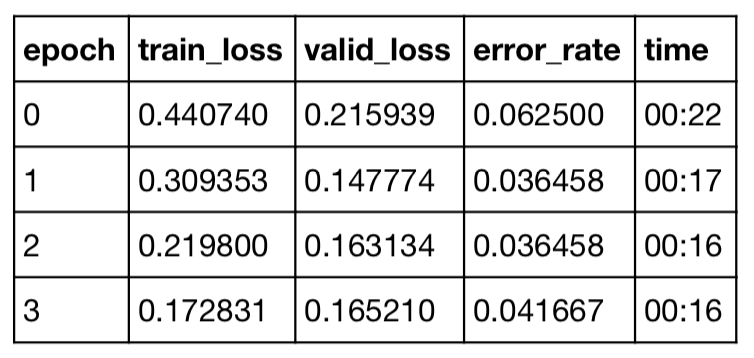
\includegraphics[width=10cm]{../images/2.png}

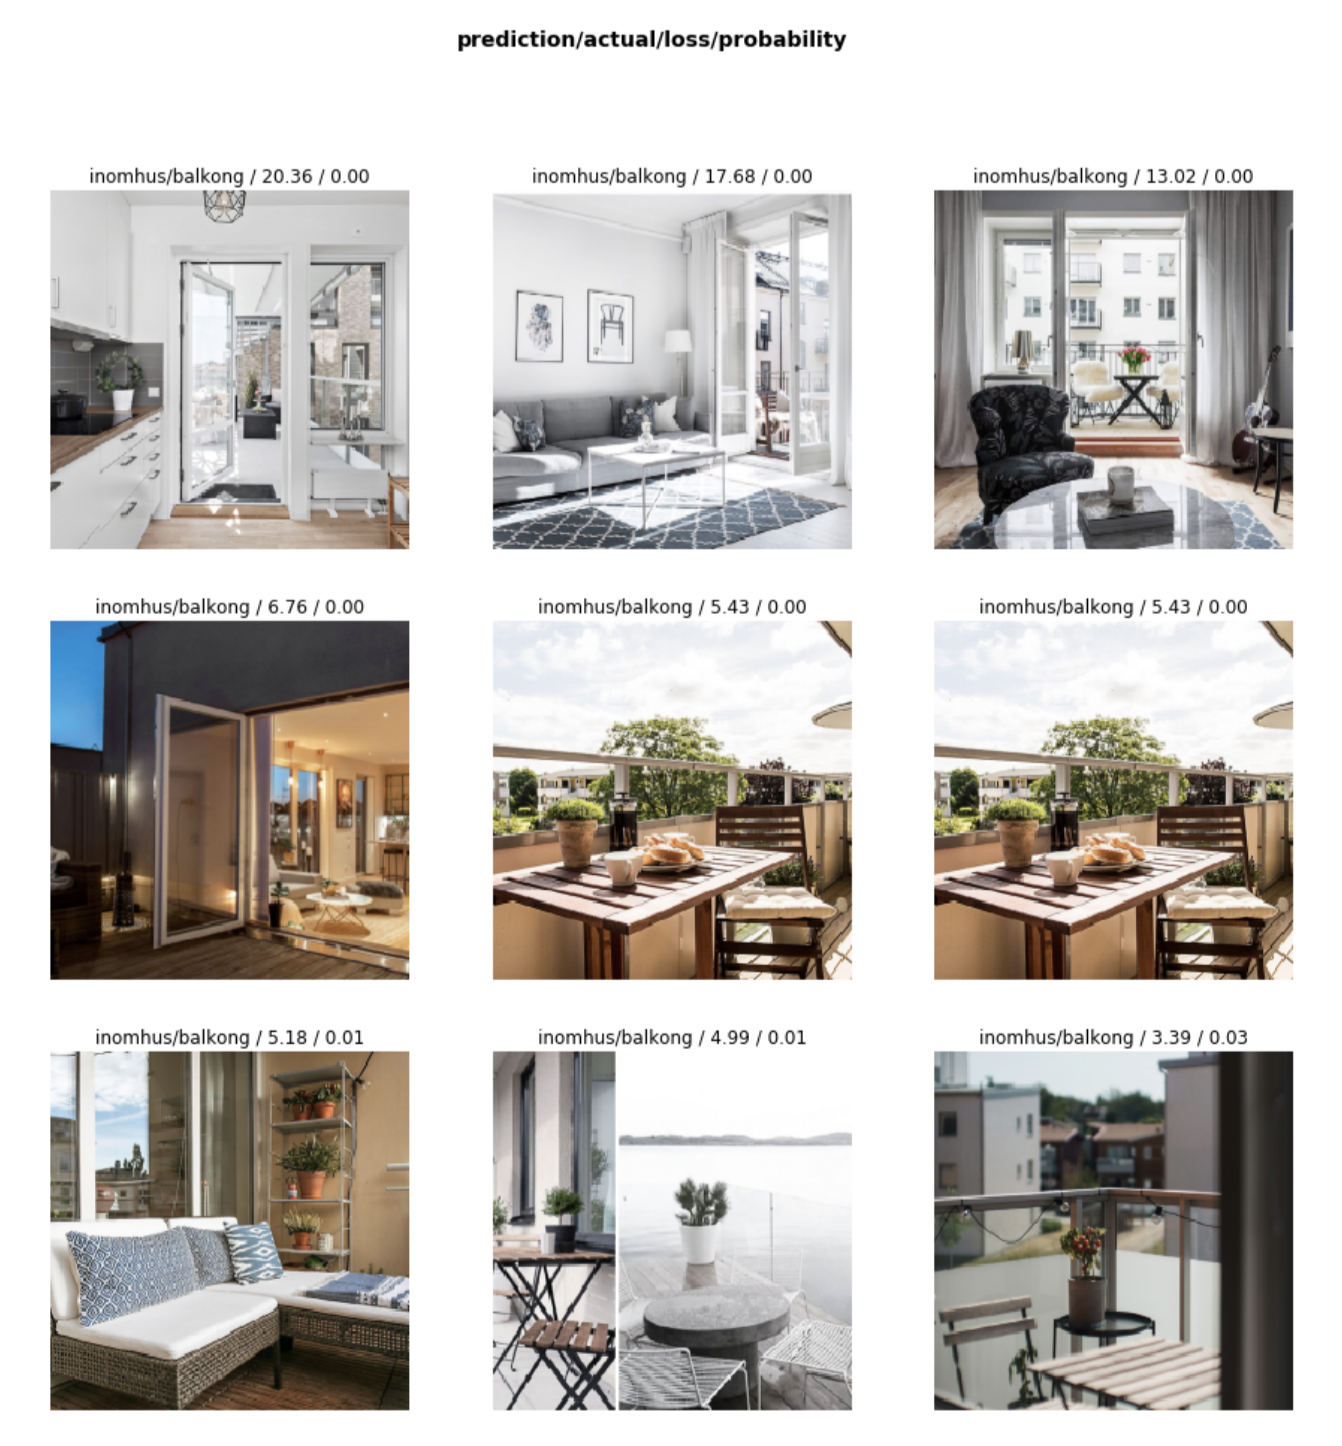
\includegraphics[width=10cm]{../images/3.png}

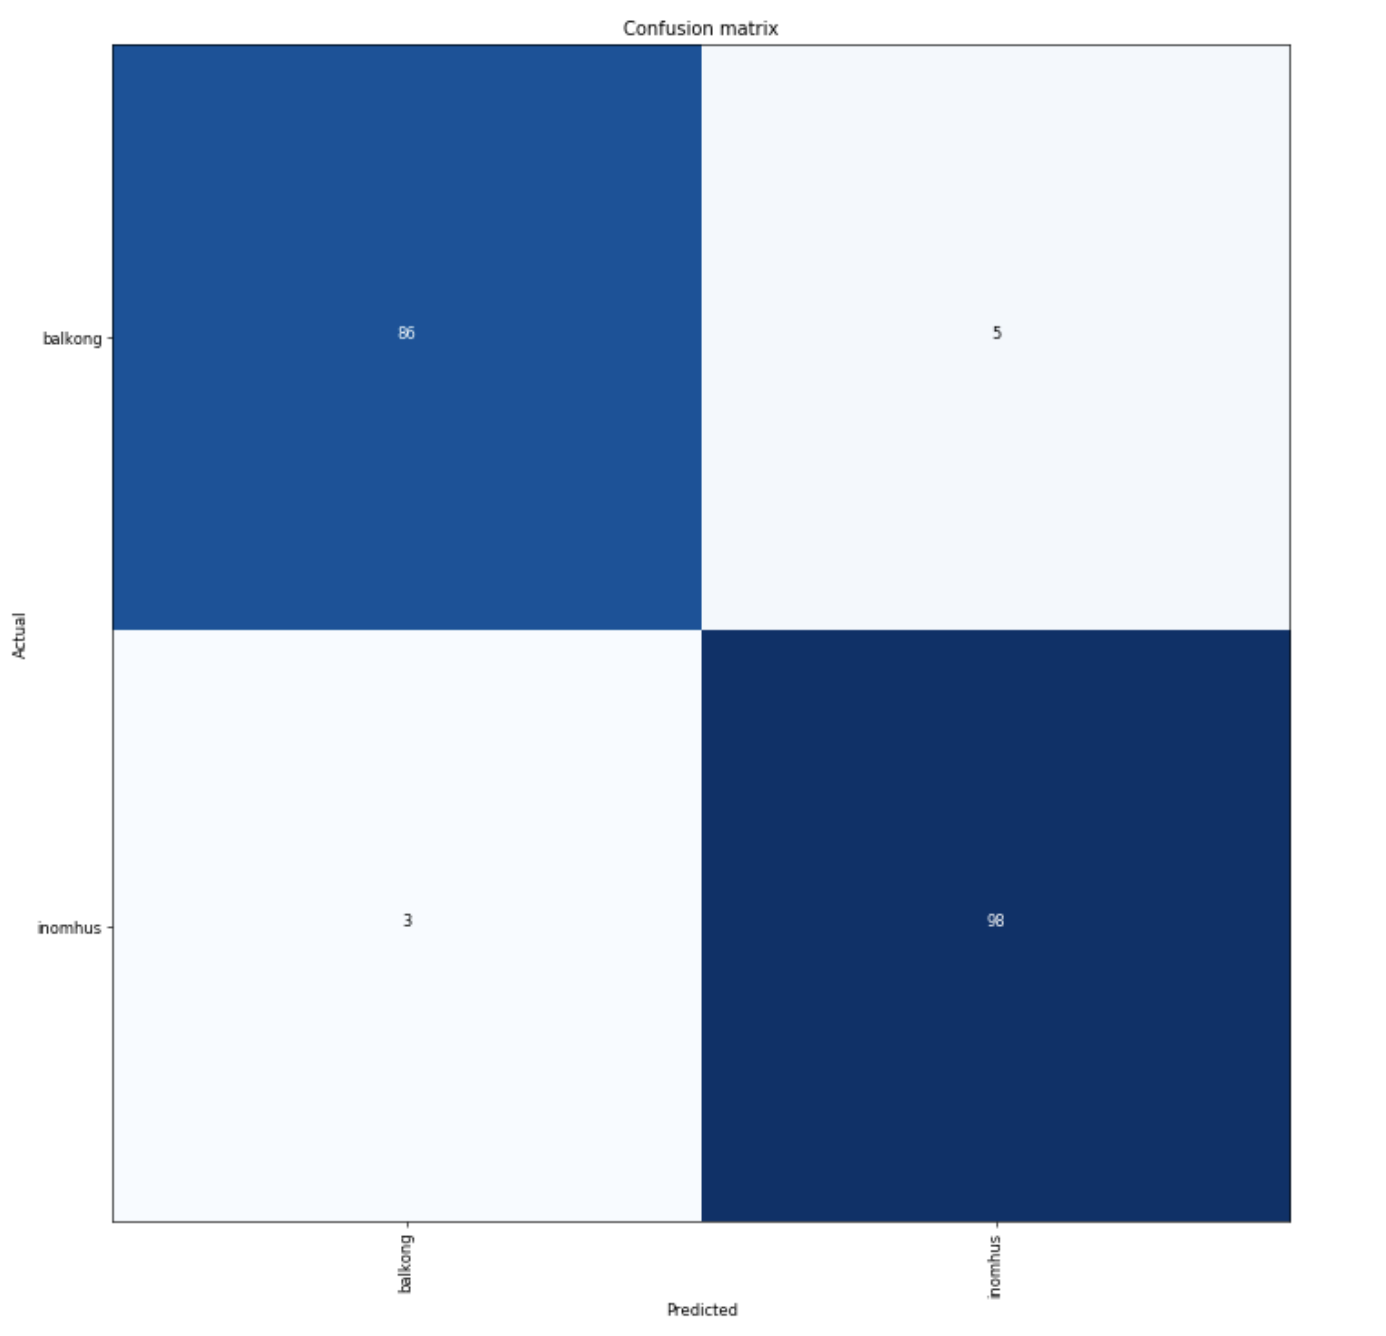
\includegraphics[width=10cm]{../images/4.png}

\chapter{Diskussion}
Diskutera resultatet och hur olika delar kan ha påverkat eller påverkade. Diskutera eventuell framtida forskning. Begränsningar med resultatet.
Etiska aspekter. Hållbarhet. 

  \section{Fortsätt forskning}
  Vid värdering så är det också intressant att få ut attribut, så kan man räkna med det i värderingskalkylen.

\chapter{Slutsats}
Slutsats av vad vi kom fram till.

\printbibliography[heading=bibintoc]
\appendix
  \chapter{Appendix A}

\tailmatter
\end{document}
